\documentclass[submit]{harvardml}

\course{CS181-S20}
\assignment{Assignment \#4}
\duedate{11:59pm March 27, 2020}

\usepackage[OT1]{fontenc}
\usepackage[colorlinks,citecolor=blue,urlcolor=blue]{hyperref}
%\usepackage[pdftex]{graphicx}
\usepackage[final]{graphicx}
%\usepackage{graphicx}
\usepackage{subfig}
\usepackage{caption}
\usepackage{fullpage}
\usepackage{soul}
\usepackage{amsmath}
\usepackage{amssymb}
\usepackage{color}
\usepackage{todonotes}
\usepackage{listings}
\usepackage{common}
\usepackage{float}


\usepackage[mmddyyyy,hhmmss]{datetime}

\definecolor{verbgray}{gray}{0.9}

\lstnewenvironment{csv}{
  \lstset{backgroundcolor=\color{verbgray},
  frame=single,
  framerule=0pt,
  basicstyle=\ttfamily,
  columns=fullflexible}}{}
 
\begin{document}

\begin{center}
{\Large Homework 4: SVM, Clustering, and Ethics}\\
\end{center}

\subsection*{Introduction}

This homework assignment will have you work with SVMs, 
clustering, and engage with the ethics lecture.  

Please submit the \textbf{writeup PDF to the Gradescope assignment `HW4'}. Remember to assign pages for each question.

Please submit your \textbf{\LaTeX\ file and code files to the Gradescope assignment `HW4 - Supplemental'}. 

You can use a \textbf{maximum of 2 late days} on this assignment.  Late days will be counted based on the latest of your submissions. 

\newpage

%%%%%%%%%%%%%%%%%%%%%%%%%%%%%%%%%%%%%%%%%%%%%
% Problem 1
%%%%%%%%%%%%%%%%%%%%%%%%%%%%%%%%%%%%%%%%%%%%%
\begin{problem}[Fitting an SVM by hand, 10pts]

  For this problem you will solve an SVM by hand, relying on principled rules and SVM properties. 
  For making plots, however, you are allowed to use a computer or other graphical tools.

Consider a dataset with the following 7 data points each with $x \in \reals$ and $y \in \{ -1, +1 \}$ : \[\{(x_i, y_i)\}_{i = 1}^7 =\{(-3 , +1) , (-2 , +1 ) , (-1,  -1 ), (0, +1), ( 1 , -1 ), ( 2 , +1 ) , (3 , +1 )\}\] Consider
mapping these points to $2$ dimensions using the feature vector $\bphi(x) =  (x, -\frac{8}{3}x^2 + \frac{2}{3}x^4 )$. The hard margin classifier training problem is:
%
\begin{align*}
  &\min_{\mathbf{w}, w_0} \|\mathbf{w}\|_2^2 \label{eq:dcp} \\
  \quad \text{s.t.} \quad & y_i(\mathbf{w}^\top \bphi(x_i) + w_0) \geq 1,~\forall i \in \{1,\ldots, n\}\notag
\end{align*}

Make sure to follow the logical structure of
the questions below when composing your answers, and to justify each step.

\begin{enumerate}
\item Plot the transformed training data in $\reals^2$ and draw the optimal decision boundary
of the max margin classifier. You can determine this by inspection (i.e. by hand, without actually doing any calculations).

\item  What is the value of the margin achieved by the optimal
decision boundary found in Part 1? 

\item Identify a unit vector that is orthogonal to the decision boundary.

\item Considering the discriminant $h(\bphi(x);\boldw,w_0)=\boldw^\top\bphi(x) +w_0$, 
give an expression for {\em all possible} $(\boldw,w_0)$ that define
the decision boundary. Justify your answer.

  \item Consider now the training problem for this dataset. Using your answers so far,
    what particular solution to $\boldw$ will be optimal for the
    optimization problem?

  \item What is the corresponding optimal value of $w_0$ for the $\boldw$ found in Part 5 (use your result from Part 4 as guidance)? Substitute in these optimal values and write out the discriminant function
    $h(\bphi(x);\boldw,w_0)$ in terms of the variable $x$ .


\item What are the support vectors of the classifier?  Confirm that
  the solution in Part 6 makes the constraints above binding for these
  support vectors.

\end{enumerate}

\end{problem}

\subsection*{Solution}

\begin{enumerate}
    \item Here is a plot of $x_2$ on the vertical axis and $x_1 = x$ on the horizontal axis. By inspection, the boundary should be at the line $x_2 = -1$, where points below are classified as negative and points above the line are classified as positive. The transformed points are $(-3,30),(-2,0),(-1,-2),(0,0),(1,-2),(2,0),(3,30)$.
    
    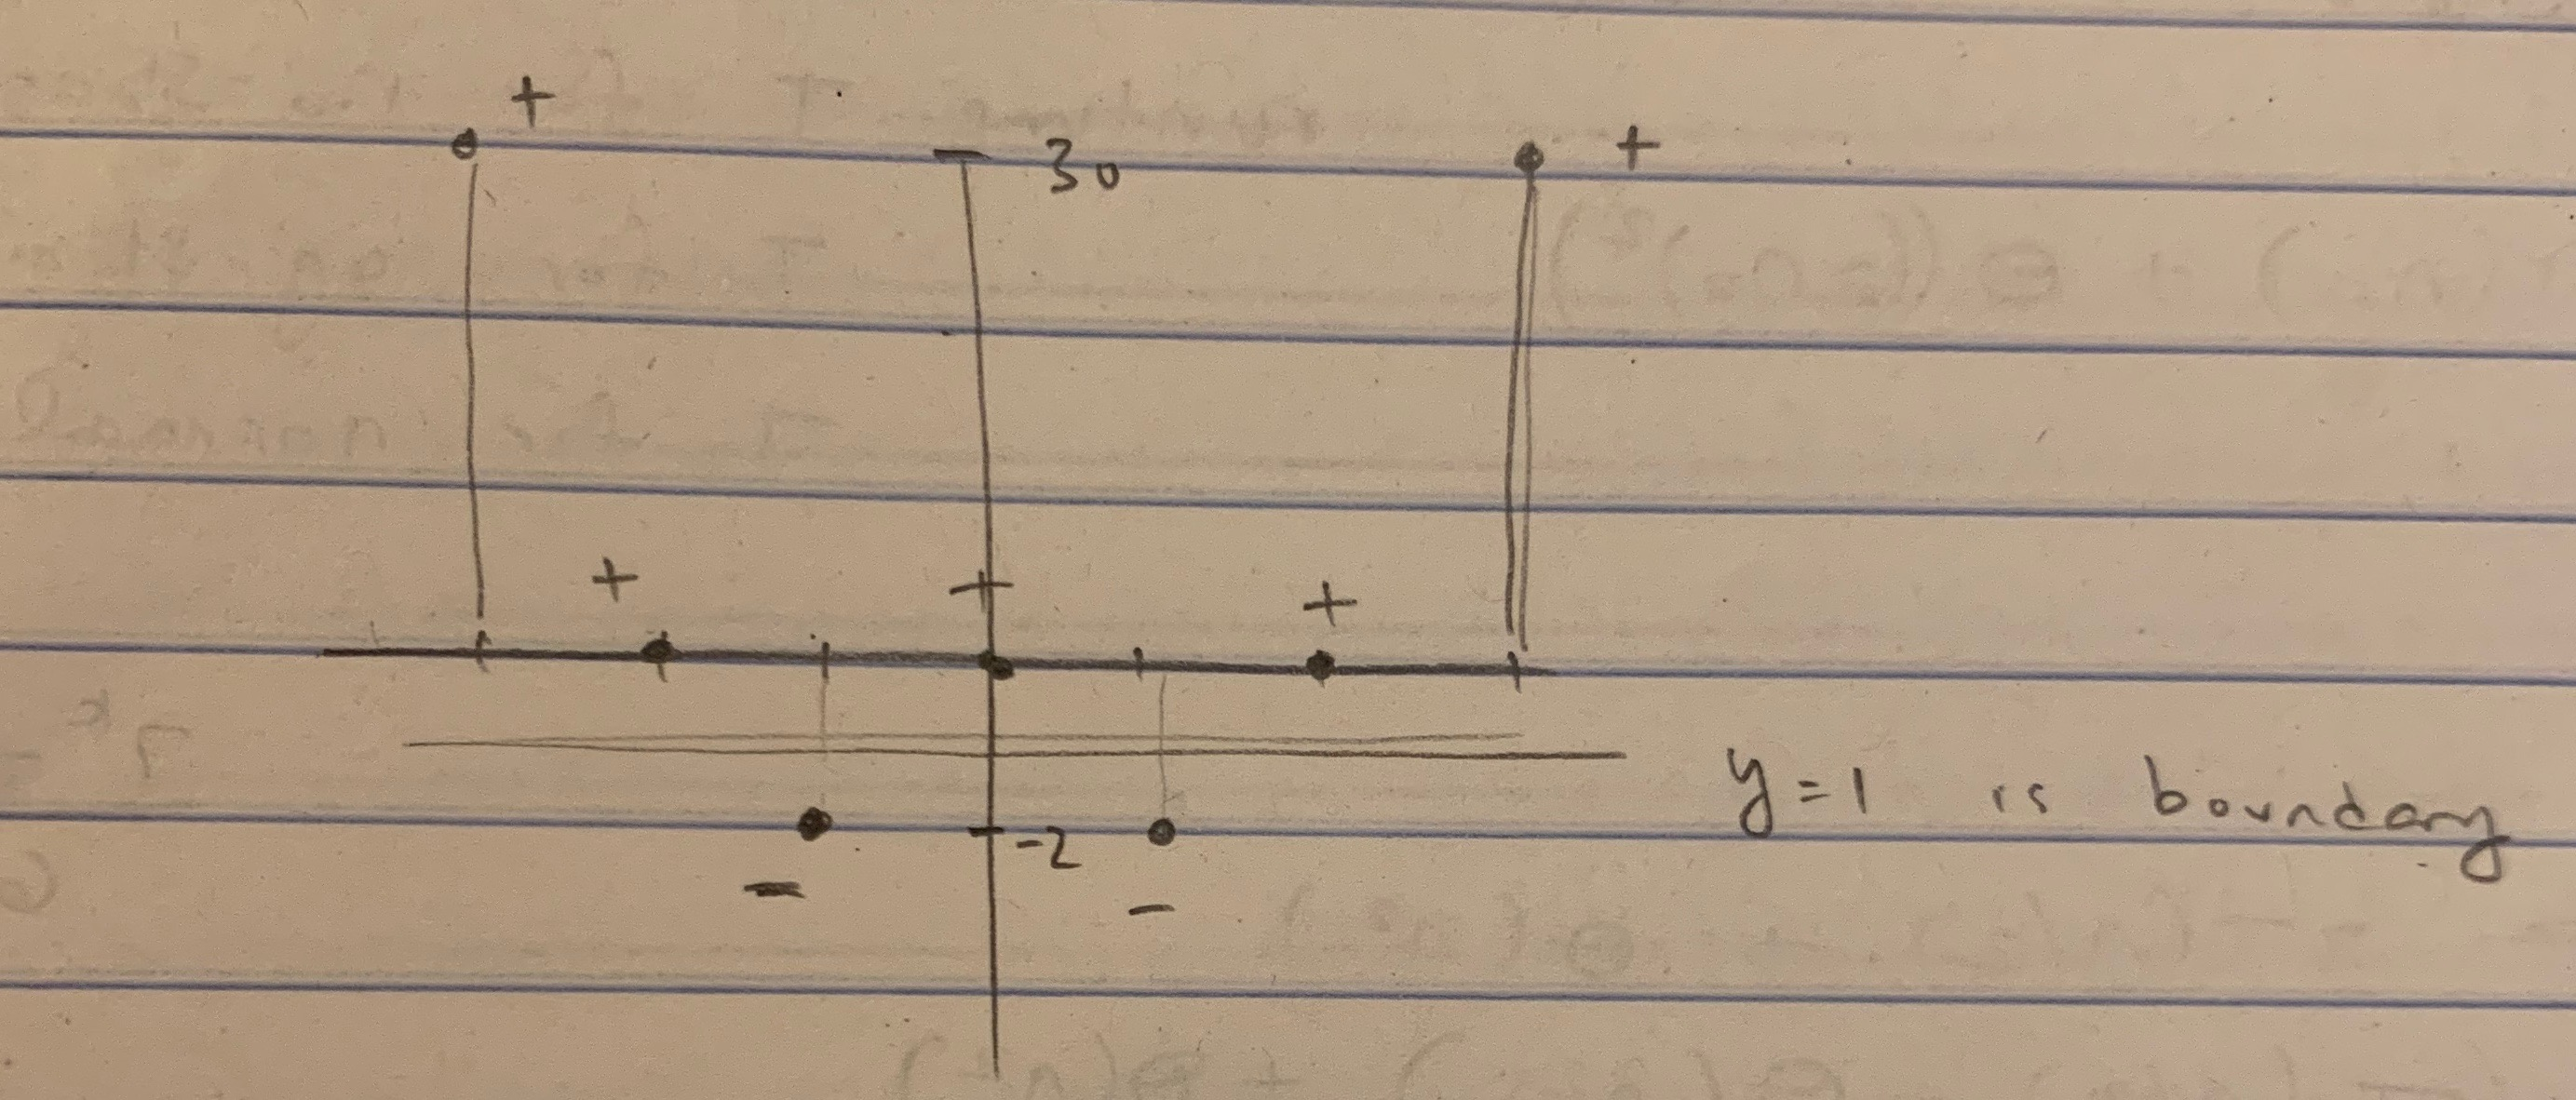
\includegraphics[width = 3in]{IMG_2052.jpg}
    
    \item The margin is the minimum distance to boundary, which is 1, since we have points at $x_2 = 0$ and $x_2 = -2$.
    
    \item Since the boundary is $x_2 = -1$, a unit vector orthogonal to that line is vertical, such as $\vec{w} = \langle 0,1 \rangle$.
    \item A point on the boundary should have margin 0, we can plug in a point $\phi(x) = p$ on the boundary $x_2 = -1$, such as $p = \langle x_1, -1 \rangle$, to solve for $\vec{w}$ and $w_0$ generally. While we know the direction of $\vec{w}$, the magnitude could be scaled by a factor of $k$, where $k$ is a positive real number. Then, we have
    \begin{align*}
        h( \phi(x) ; w, w0) = w^T \phi(x) + w_0 &= 0 \\
        k \langle 0,1 \rangle \cdot \langle x_1, -1 \rangle + w_0 &= 0 \\
        -k + w_0 &= 0 \implies w_0 = k.
    \end{align*}
    Then, a general solution for $(\boldw, w_0)$ is $\boldw = \langle 0, k \rangle$ and $w_0 = k$ for $k > 0$.
    \item Now, plugging a support vector should give us $y_n(\boldw^T \phi(x_n) + w_0) = 1$. We can plug in the support vector $(-1,-2)$ and see
    \begin{align*}
        -1(k \langle 0,1 \rangle \cdot \langle -1,-2 \rangle + k) &= 1 \\
        k(-2) + k &= -1 \\
        k(-1) &= - 1 \implies k = 1,
    \end{align*}
    so the optimal solution is $\boldw = \langle 0, 1 \rangle$ and $w_0 = 1$.
    
    \item Since $\boldw = \langle 0,k \rangle = \langle 0, 1 \rangle$ and $w_0 = k = 1$, we have that the discriminant is $h(\phi(x) ; \boldw, w_0) = \langle 0, 1 \rangle^T \phi(x) + 1$. 

    \item The support vectors are $(x_i, y_i) = (-2, +1), (-1, -1), (0,+1),(1,-1),(2,+1)$, which give us $\phi(x_i) = (-2, 0), (-1,-2), (0,0), (1,-2), (2,0)$. Let us verify that $y_n ( \langle 0,1 \rangle \cdot \phi(x_n) + 1) = 1$ for all support vectors.
    \begin{align*}
        (-2,0)& \implies +1 (0 + 1) = 1 \\
        (-1,-2)& \implies -1(-2 + 1) = 1 \\
        (0,0)& \implies +1(0 + 1) = 1 \\
        (1,-2)& \implies -1(-2 + 1) = 1 \\
        (2,0)& \implies +1(0 + 1) = 1
    \end{align*}
\end{enumerate}


% \newpage

%%%%%%%%%%%%%%%%%%%%%%%%%%%%%%%%%%%%%%%%%%%%%
% Problem 2
%%%%%%%%%%%%%%%%%%%%%%%%%%%%%%%%%%%%%%%%%%%%%

\begin{problem}[K-Means and HAC, 20pts]


For this problem you will implement K-Means clustering and HAC from
scratch. Using \texttt{numpy} is fine, but don't use a third-party
machine learning implementation like \texttt{scikit-learn}. You will
then apply this approach to the clustering of image data.

We've provided you with a subset of the MNIST dataset, a collection of
handwritten digits used as a benchmark for image recognition (you can
learn more about the data set at
\url{http://yann.lecun.com/exdb/mnist/}). The MNIST task is widely
used in supervised learning, and modern algorithms do very well.

Here you will apply unsupervised learning to MNIST. You have been given
representations of MNIST images, each of which is a $784\times1$
greyscale handwritten digit from 0-9. Your job is to implement K-means
clustering and HAC on MNIST, and to test whether these relatively
simple algorithms can cluster similar-looking images together.

The code given in \texttt{T4\_P2.py} loads the images into your environment into two arrays -- \texttt{large\_dataset} is a 5000x784 array that should be used for K-means, while \texttt{small\_dataset} is a 300x784 array that will be used for HAC clustering. In your code, you should use the $\ell_2$ norm (i.e. Euclidean distance) as your distance metric.

\textbf{Important:} Remember to include all of your plots in your PDF submission!

\begin{enumerate}

\item Starting at a random initialization and $K = 10$, plot
  the K-means objective function (the residual sum of squares) as a function of iterations and verify
  that it never increases.

\item Run the K-means algorithm for 5 different restarts for different
  values of $K$, setting $K = 5, 10, 20$. Plot the final K-means objective value as a function
  of $K$ with error bars over the $5$ random restarts. To clarify, your
  x-axis will be $K$, your y-axis will be the average objective function value
  after your algorithm converges, and each data point will have an
  error bar -- to calculate these error bars you must run your K-means
  algorithm $5$ times for each $K$ (giving you multiple final objective values
  for each $K$) then use these values to calculate a standard deviation for
  each $K$ before plotting error bars around each data point. How
  does the final value of the objective function and the standard deviation of the final
  value of the objective function change with $K$? (Note: Our code takes ~10 minutes to run for this Part)
  
\item For $K=10$ and for 5 random restarts, show the mean
  image (aka the centroid) for each cluster.
  To render an image, use the pyplot
  \texttt{imshow} function. There should be 50 total images. Include all of these images
  as part of a single plot (e.g. don't have 50 pages in your write-up with a
  separate image on each page).

\item Repeat Part 3, but first standardize the data. That is, center
  the data before running K-means on it, such that each pixel has mean 0 and variance 1 (except
  for any pixels that have zero variance, for these you can simply
  divide by 1). For $K=10$ and 5 random restarts, show the mean image
  (aka the centroid) for each cluster. There should be 50 total
  images. Again, include all of these images as part of a single plot.
  Compare these images to those from Part 3.

\item Implement HAC for min, max, and centroid-based linkages. Fit these models to the \texttt{small\_dataset} images. 
  For each of these 3 linkage criteria, find the mean image for each cluster when using $10$ clusters, and display these images on a plot. There should be 30 total images.
  How do these mean images compare to those found with K-means? \textbf{Important Note:} For this part only, you may use the \texttt{scipy} package's \texttt{cdist} function to calculate the Euclidean distances between every pair of points in two arrays. DO NOT use \texttt{scipy} for anything else. 

\item For each of the 3 HAC linkages (max/min/centroid), make a plot of
  ``Distance between most recently merged clusters" (y-axis) v. ``Total number of merges completed" (x-axis).
  Does this plot suggest that there are any  natural cut points? 

\item Re-fit a K-means with $K = 10$ model and HAC min/max/centroid models using $10$ clusters on the \texttt{small\_dataset} images. Use the \texttt{seaborn} module's \texttt{heatmap} function to plot a confusion matrix of clusters v. actual digits, i.e. the cell at the $i$th row, $j$th column of your confusion matrix should be the number of times that an image with the true label of $j$ appears in cluster $i$. How well do the different approaches match the digits? Is this matching a reasonable evaluation metric for the clustering?  Explain why or why not.  
  
\end{enumerate}

\end{problem}

\subsection*{Solution}

\begin{enumerate}
    %1
    \item We plot the K-means objective function below (Loss vs. Iterations). It is indeed decreasing!
    
    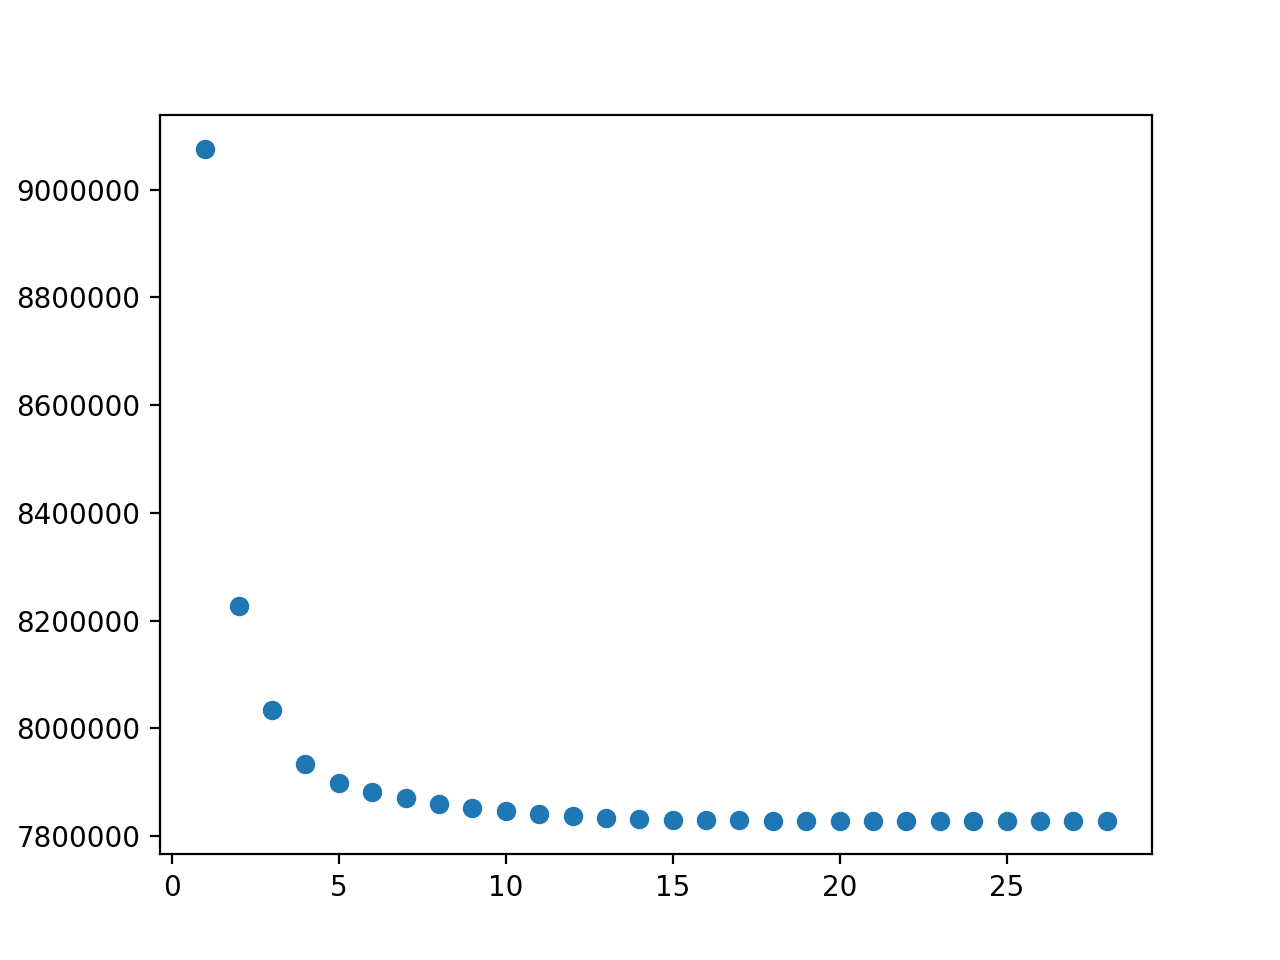
\includegraphics[width=0.5\linewidth]{Kmeans_Loss_3.png}
    
    %2
    \item We plot the final K-means objective value as a function of $K$ with error bars below. The final value of the objective decreases with $K$ as expected, since more clusters means that points will be on average closer to a cluster center. We also observed that the standard deviation also seems to decrease slightly, which makes sense since more clusters means that there is less room for variation for the cluster.
    
    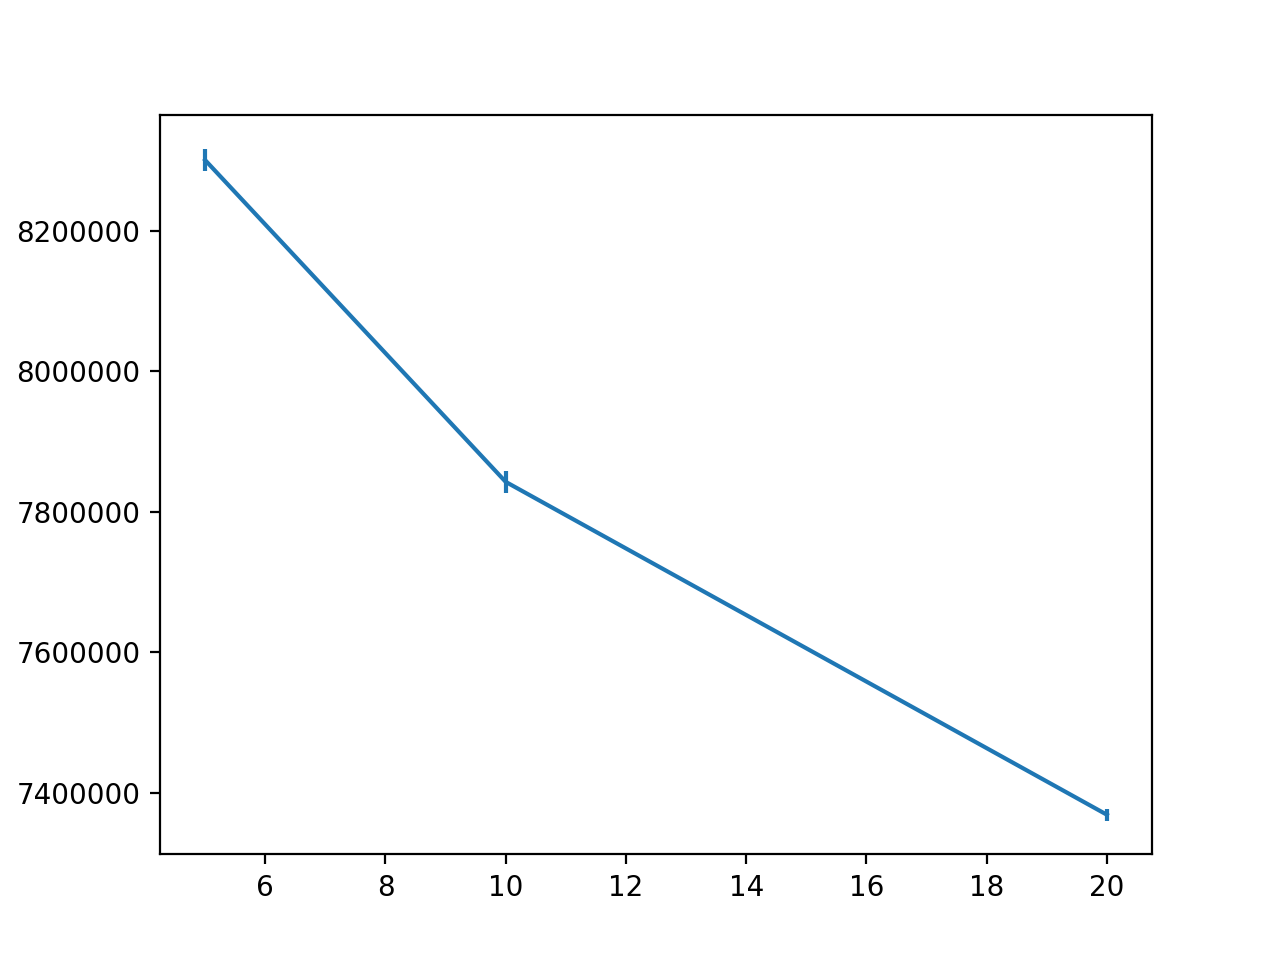
\includegraphics[width=0.5\linewidth]{Errorbars_A.png}
    \newpage 
    %3
    \item Figure \ref{fig:kmeans} shows the cluster centers for $K = 10$ and 5 random restarts.

    \begin{figure}[H]
    \centering
    \subfloat[Init 1]{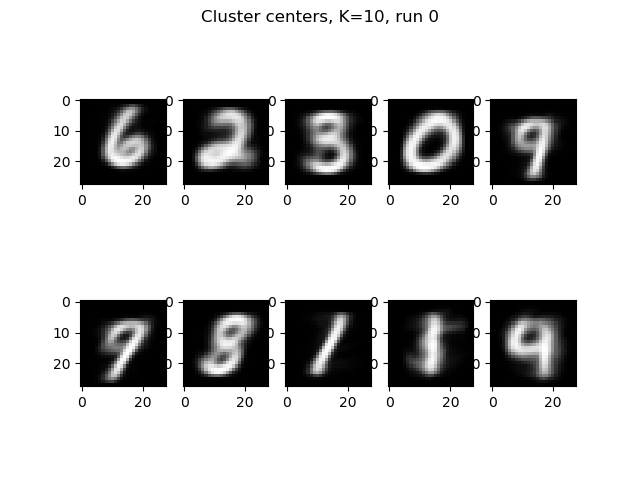
\includegraphics[width=0.33\linewidth]{kmeans_centers_k10_run0.png}}
    \subfloat[Init 2]{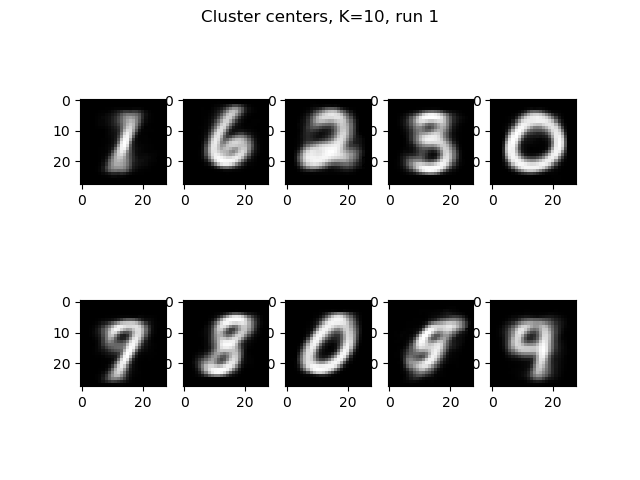
\includegraphics[width=0.33\linewidth]{kmeans_centers_k10_run1.png}}
    \subfloat[Init 3]{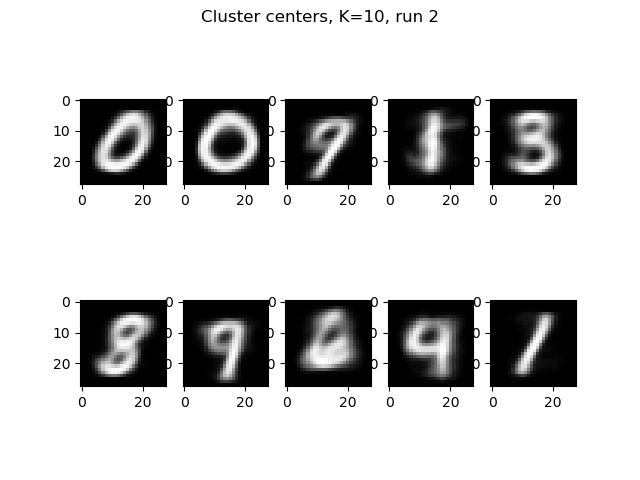
\includegraphics[width=0.33\linewidth]{kmeans_centers_k10_run2.png}} \\
    \subfloat[Init 4]{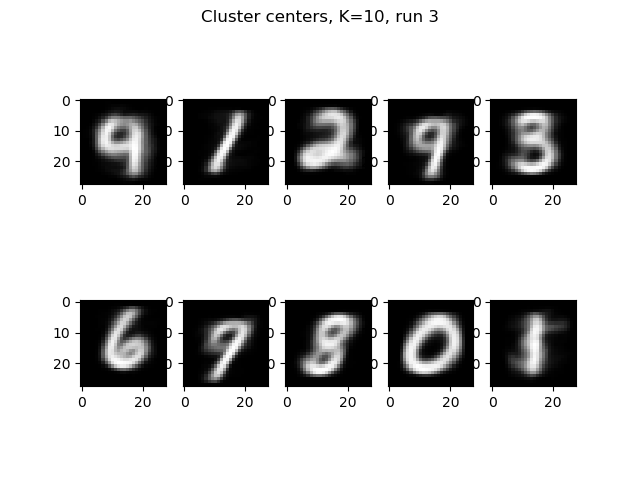
\includegraphics[width=0.33\linewidth]{kmeans_centers_k10_run3.png}}
    \subfloat[Init 5]{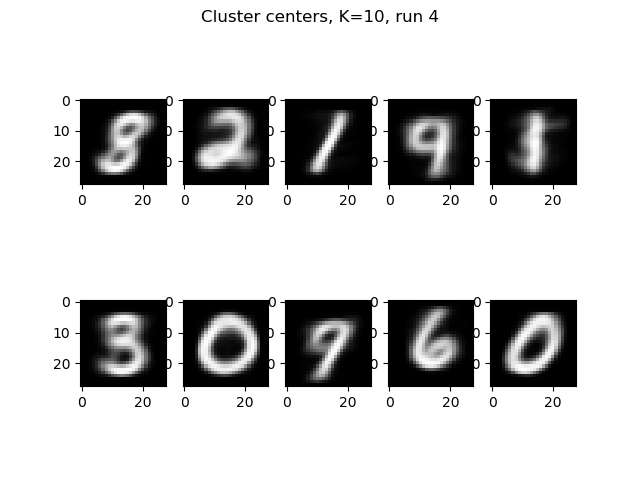
\includegraphics[width=0.33\linewidth]{kmeans_centers_k10_run4.png}}
    \caption{K-Means Cluster Centers for 5 Random Restarts}
    \label{fig:kmeans}
    \end{figure}
    
    %4
    \newpage
    \item We first standardize the data, then plot the cluster centers below in Figure \ref{fig:norm}. Because of the normalization, some of the pixels are varying shades of gray instead of black. The digits themselves do look pretty clear, which means the clustering algorithm does quite well, just as well as the normal K-Means if not better.
    
    \begin{figure}[H]
    \centering
    \subfloat[Init 1] {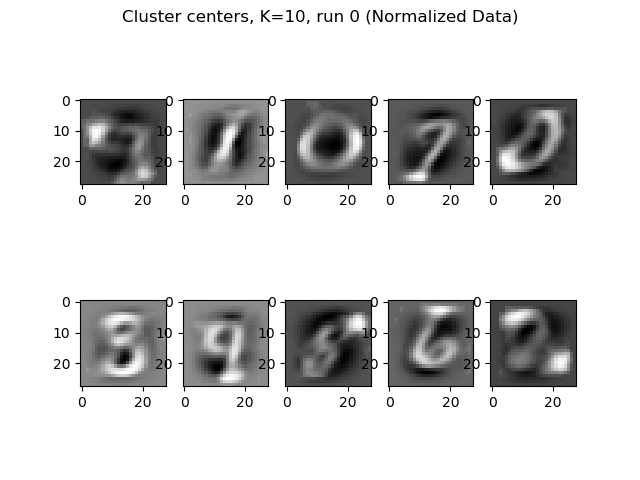
\includegraphics[width=0.33\linewidth]{kmeans_centers_normed_k10_run0.png}}
    \subfloat[Init 2] {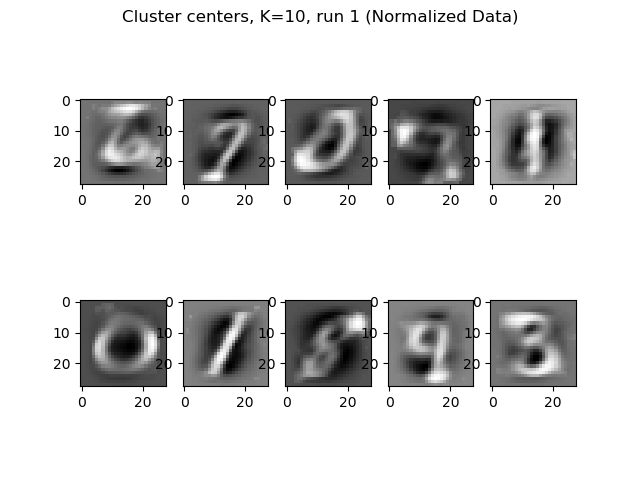
\includegraphics[width=0.33\linewidth]{kmeans_centers_normed_k10_run1.png}}
    \subfloat[Init 3] {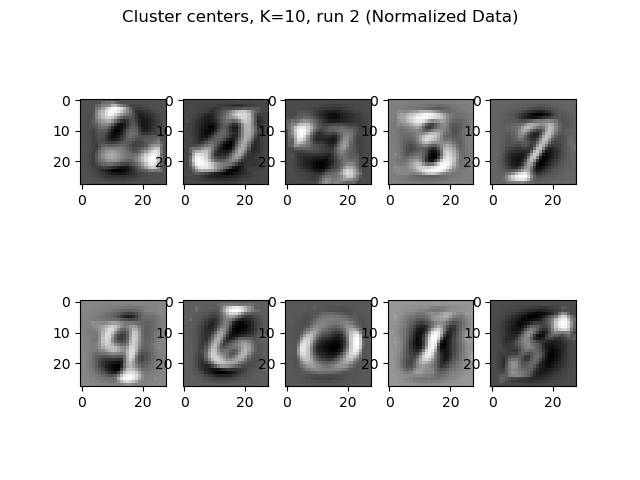
\includegraphics[width=0.33\linewidth]{kmeans_centers_normed_k10_run2.png}} \\
    \subfloat[Init 4] {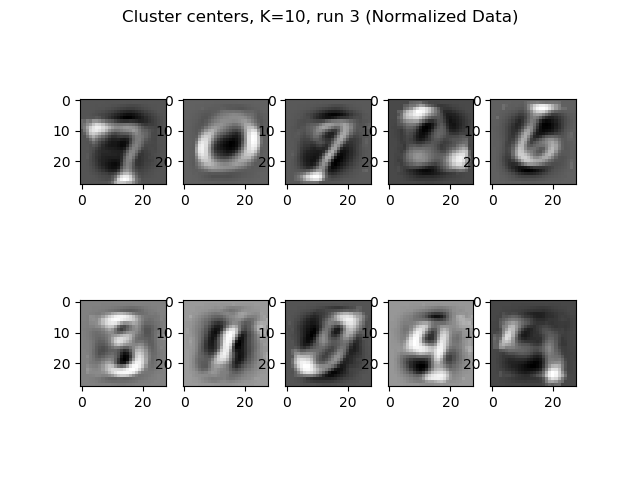
\includegraphics[width=0.33\linewidth]{kmeans_centers_normed_k10_run3.png}}
    \subfloat[Init 5] {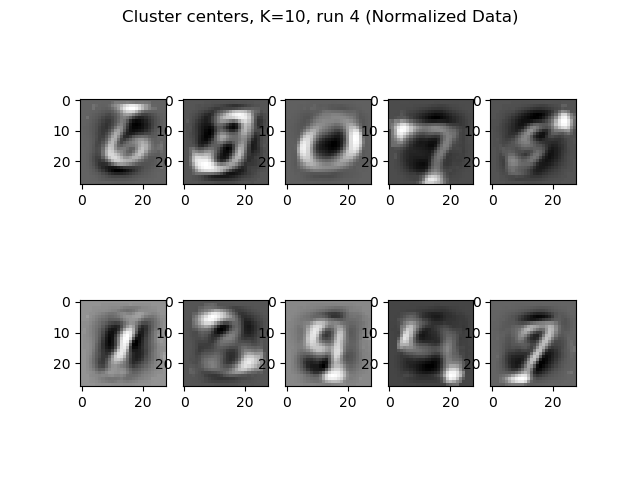
\includegraphics[width=0.33\linewidth]{kmeans_centers_normed_k10_run4.png}}
    
    \caption{Cluster Centers for K-Means after Normalized Data, 5 Random Initializations}
    \label{fig:norm}
    \end{figure}
    
    %5
    \item Figure \ref{fig:HAC} shows the cluster centers produced by HAC with min, max, and centroid-based linkages. Comparing the HAC images to the K-Means images, we can see that HAC results for all three linkages appear worse than K-Means. Specifically, the HAC clusters are less able to pick out true digits. Many clusters seem blurrier than K-Means, and some clusters are too blurry to even look like a digit, likely because those clusters contain images of multiple digits.
    
    \begin{figure}[H]
    \centering
    \subfloat[Min-Linkage HAC] {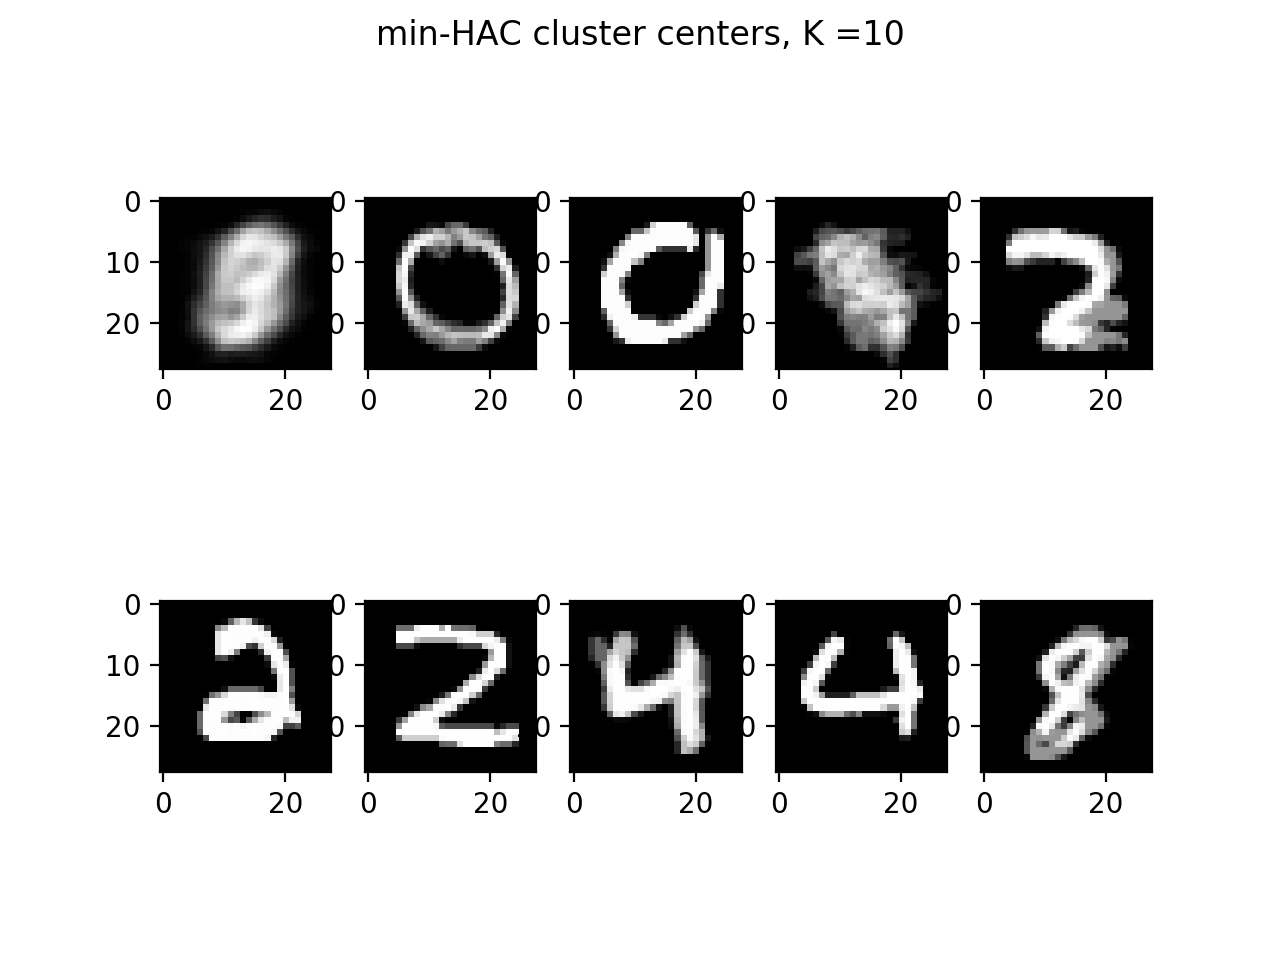
\includegraphics[width=0.33\linewidth]{min_hac_clusters_A.png}}
    \subfloat[Max-Linkage HAC] {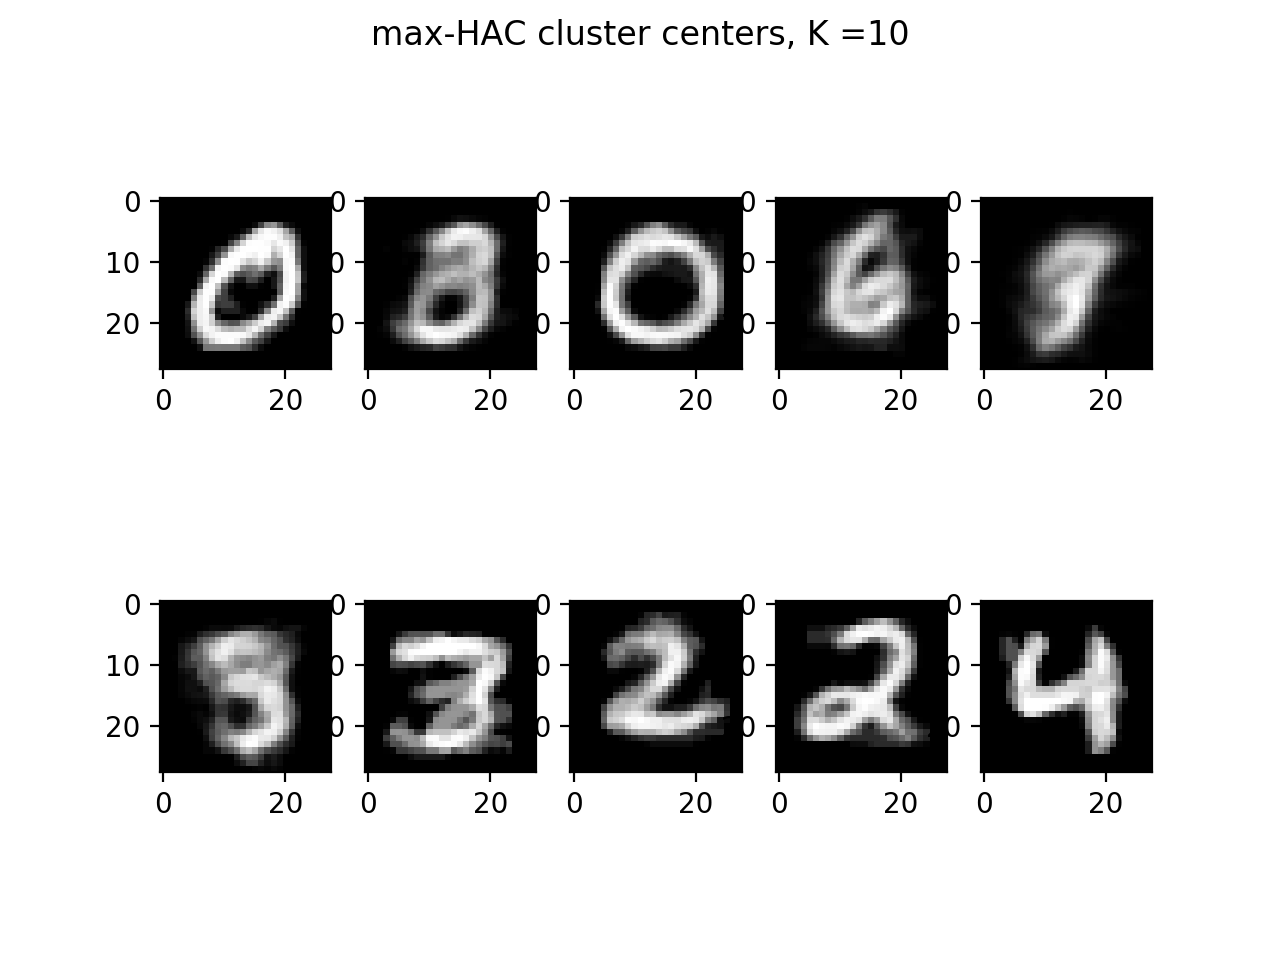
\includegraphics[width=0.33\linewidth]{max_hac_clusters_A.png}}
    \subfloat[Centroid-Linkage HAC] {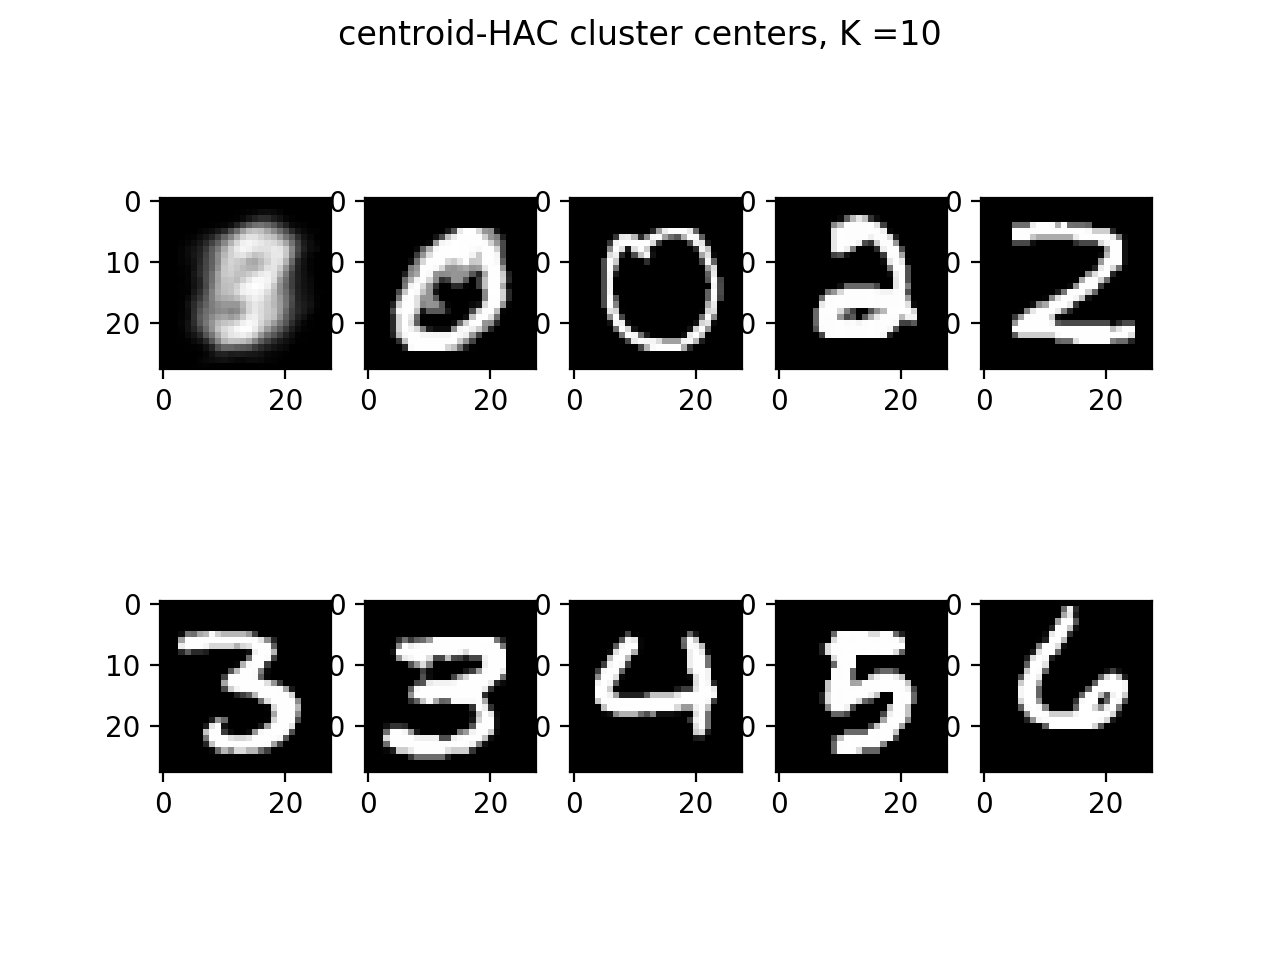
\includegraphics[width=0.33\linewidth]{centroid_hac_clusters_A.png}}
    
    \caption{Cluster Centers for HAC}
    \label{fig:HAC}
    \end{figure}
    
    %6
    \item Figure \ref{fig:HAC-dist} shows the 3 distance vs. merges plots. The plots do suggest natural cut points! The cut point appears to be close to 300 or between 250 and 300 for all three graphs. The distance keeps increasing as number of merges increases, and at some point approximately around 275, the distance starts increasing much faster (the slope of the graph becomes greater). This suggests that the clusters merged at the end after 275 iterations are far apart; perhaps they do not actually naturally belong to the same cluster, and the HAC is simply forcing them to be merged together.
    \begin{figure}[H]
    \centering
    \subfloat[Min-Hac Distance vs. \#Merges]{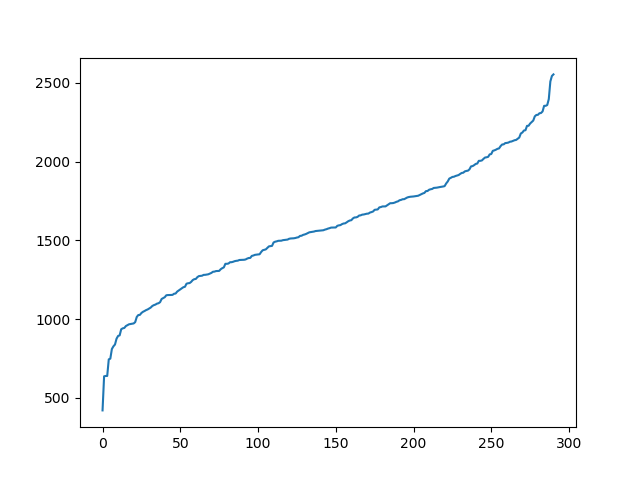
\includegraphics[width=0.3\linewidth]{min_hac_distance_vs_merge.png}}
    \subfloat[Max-Hac Distance vs. \#Merges]{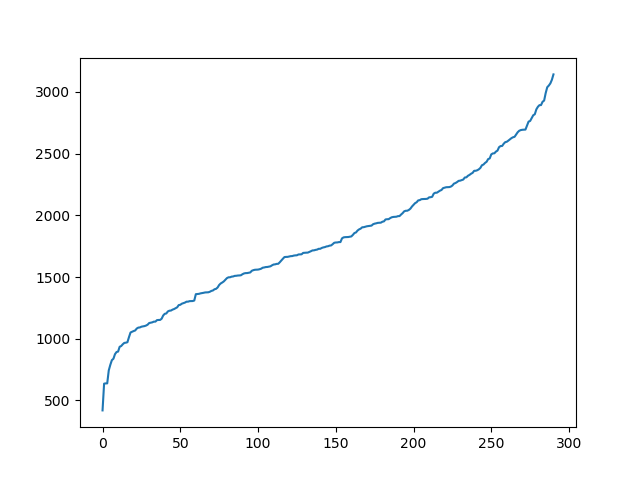
\includegraphics[width=0.3\linewidth]{max_hac_distance_vs_merge.png}}
    \subfloat[Centroid-Hac Dist vs. \#Merges] {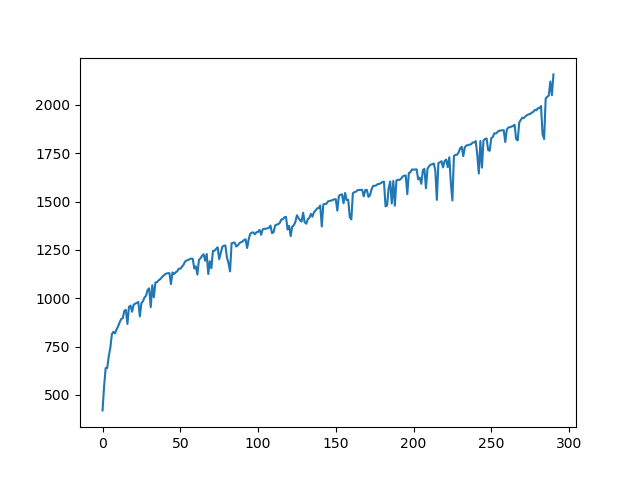
\includegraphics[width=0.3\linewidth]{centroid_hac_distance_vs_merge.png}}
    \caption{Cluster Centers for 5 Restarts}
    \label{fig:HAC-dist}
    \end{figure}
    
    \item Here are the confusion matrices for the four clustering methods (Figure \ref{fig:heatmaps}). We can tell that K-Means and Max-HAC cluster the digits better than Min-HAC and Centroid-HAC, with K-Means doing the best and Centroid-HAC doing the worst. In a perfect clustering, we would see mostly dark heatmaps with 10 light squares, one light square per row (meaning that each cluster picked up on a single and distinct true label).
    
    We see that K-means is pretty good, for example, cluster 5 cleanly picks out the digit 6, cluster 4 strongly picks out the digit 8, and cluster 9 picks out the digit 0, etc. Each row usually has one very light square, and sometimes a couple kind-of light squares, but overall, the clusters identify digits well.
    
    Max-HAC has some good clusters, such as cluster 3 which picked out the digit 6, but it also has poor clusters, such as 8 and 9 which didn't pick up any digits. Cluster 4 seems to pick out 1s well but also picks up additional noise from other digits.
    
    On the other hand, the bright row in cluster 0 indicates that Min-HAC and Centroid-HAC seem to just drop most digits into one cluster while leaving few data points to the other clusters.
    
    Examining the confusion matrix heatmaps of assigned cluster vs. true label in this way is a pretty reasonable evaluation metric for clustering. We can tell how consolidated or noisy the clustering was based on the patterns of light squares. Essentially, we can see how close the result is to a perfect clustering.
    \begin{figure}[H]
    \centering
    
    \subfloat[Confusion Matrix for K-Means Classifier] {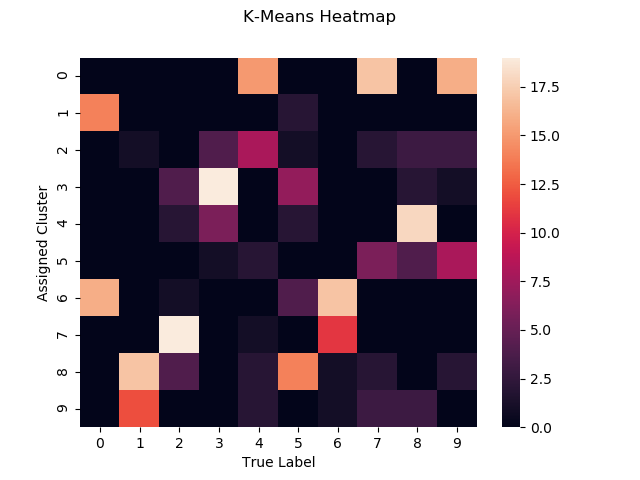
\includegraphics[width=0.4\linewidth]{kmeans_confusion.png}}
    \subfloat[Confusion Matrix for Min-HAC] {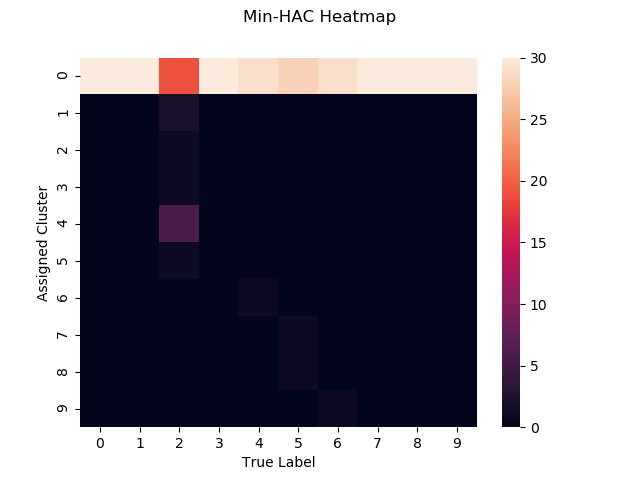
\includegraphics[width=0.4\linewidth]{hac_min_confusion.png}} \\
    \subfloat[Confusion Matrix for Max-HAC] {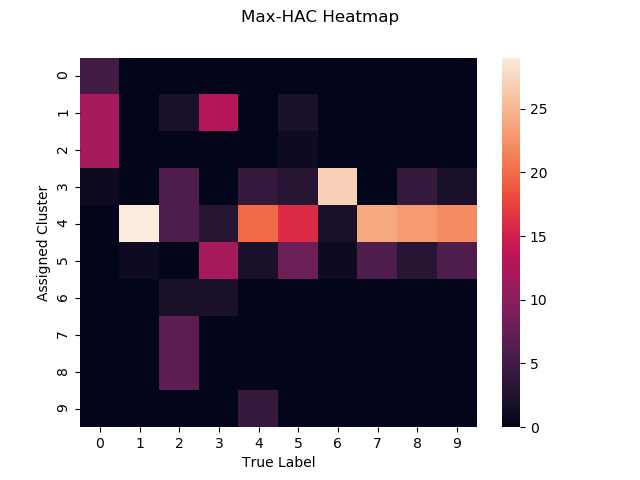
\includegraphics[width=0.4\linewidth]{hac_max_confusion.png}}
    \subfloat[Confusion Matrix for Centroid-HAC] {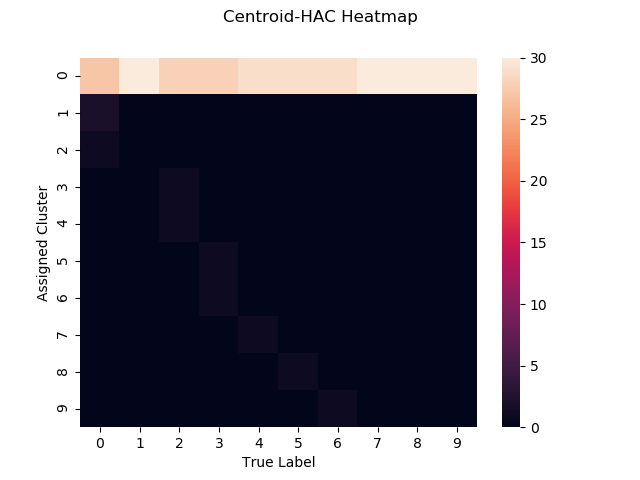
\includegraphics[width=0.4\linewidth]{hac_centroid_confusion.png}}
    
    \caption{Confusion Matrix Heatmaps for Four Clustering Methods}
    \label{fig:heatmaps}
    \end{figure}
    
    
\end{enumerate}

\pagebreak
%%%%%%%%%%%%%%%%%%%%%%%%%%%%%%%%%%%%%%%%%%%%%
% Problem 3
%%%%%%%%%%%%%%%%%%%%%%%%%%%%%%%%%%%%%%%%%%%%%
\begin{problem}[Ethics Assignment, 15pts]
Imagine that you are a product manager in a technology company and the board of directors requests a detailed report of the potential social impact of the product you're building. You are currently working on an algorithm designed to allocate economic resources for various health providers. You are instructed to address various kinds of possible impacts, giving special attention to the algorithm’s potential to wrongfully discriminate against vulnerable populations. 

Having followed the coding process closely, you can confidently assume that there is no discriminatory intent animating the design.  In fact, the product’s design is based on the notion that resources should be distributed to health centers in a manner that is proportional to the needs of the populations they attend to. However, you worry that there may still be wrongful discrimination due to disparate negative impact on members of low-income populations, migrants, and racial minorities. 

What further questions must you address in order to confidently determine whether the algorithm wrongfully discriminates against members of these groups? Write two questions and, for each, write a short paragraph explaining how addressing this question can help you assess the algorithm’s potential for wrongful discrimination.


We expect clear, concise, and thoughtful engagement with this question, which includes providing your reasoning for your answers.  In your response, depth is more important than breadth. We do \emph{not} expect you to do any outside research, though we encourage you to connect to lecture materials where relevant.

\end{problem}

\subsection*{Solution}

The goal of the algorithm should be to allocate economic resources for various health providers fairly. By fair, we mean it allocates proportional to the needs of the populations, without wrongful discrimination, especially not against protected categories. Even though there is no disparate treatment since intent was good, there is the possibility of unintentional disparate impact. In order to determine whether the algorithm will be fair, we should comprehensively consider a couple of questions:

Will the algorithm learn just decisions from our input data? While algorithms themselves are objective and quantitative (this may seem to be fair), the input data influences the resulting model hugely and could produce unintended unfair results. We want to make sure that the model is not picking up on an unintended proxy for prediction. For example, if we train a model based on how resources have been allocated in the past, we should ask ourselves, \textbf{is the past history of resource allocation a fair set of training labels?} Perhaps wealthier regions have always used more resources; then a model trained on these set of labels would learn to allocate more resources to wealthier resources instead of true need, only to reinforce existing biases in data, creating a feedback loop that exacerbates epistemic problem of wealth inequality. 

How do you decide which person or which population is more in need? Answering these questions will help us ensure that our training labels are fair. And that the result from training does not wrongfully discriminate. Our model inevitably needs to discriminate between healthcare providers in order to decide how much to allocate, but we don’t want to wrongfully discriminate against certain populations. In particular, we should take steps to check, \textbf{is our training data biased?} Take the current COVID-19 outbreak as an example, where your goal is sending resources to the most at-risk populations. However, predicting where COVID-19 will hit hardest (and therefore, where to send resources) is extremely difficult given the incomplete and biased data that we have on the current situation. For example in South Korea, the outbreak spread rapidly through the Shincheonji Church where a lot of members who interact with each other are young women in their 20s–30s. In response, more and more Shincheonji Church members were tested, further biasing the number of COVID-19 cases to over-represent young women. Then, the data might strongly suggest that young women are most at risk for getting COVID-19, when in reality the people around them whom they spread the disease to might be less likely to get tested but more at risk. This might then hypothetically divert resources away from elderly populations who need resources more but weren't as rigorously tested.


\newpage
%%%%%%%%%%%%%%%%%%%%%%%%%%%%%%%%%%%%%%%%%%%%%
% Name and Calibration
%%%%%%%%%%%%%%%%%%%%%%%%%%%%%%%%%%%%%%%%%%%%%
\subsection*{Name}
Katherine Tian

\subsection*{Collaborators and Resources}
Whom did you work with, and did you use any resources beyond cs181-textbook and your notes?

\subsection*{Calibration}
Approximately how long did this homework take you to complete (in hours)? 
20
\end{document}

